\chapter{Spezielle Methoden im Deep Learning}
Bereits zu Beginn (siehe Kapitel \ref{ch:DeepLearning}), wie auch im vergangenen Kapitel \ref{ch:cnn_model} wurde darauf hingewiesen, dass Convolutional Neural Networks (CNNs) allgemeinen Multilayer Perceptrons (MLPs) in zwei zentralen Punkten überlegen sind. So reduzieren sie das Problem des \textit{Overfittings}, wobei es sich um die Überanpassung des Modells an die Trainingsdaten mit dem Resultat schlechter Generalisierung auf neue unbekannte Daten handelt. Dies geschieht durch Reduktion der zu lernenden Gewichte und Verbindungen. Des Weiteren erlauben CNNs die lokale Extraktion von Merkmalen durch Einbezug räumlicher Korrelationen im Eingaberaum (vgl. \cite{LeCun1998}). 

Auch durch die Verwendung von CNNs bleiben dennoch zentrale Schwierigkeiten im Deep Learning bestehen:
\begin{itemize}
\item Verschwinden des Gradienten (\textit{Vanishing Gradient}) in tiefen Netzen (vgl. \cite{Hochreiter1991})
\item Gradientenabstieg bei nicht-konvexer Zielfunktion (vgl. \cite{Martens2010} und \cite{Dauphin14})
\item \textit{Overfitting} bei großen Netzen, insbesondere in nachgeschalteten MLPs (vgl. \cite{Hinton2012})
\item Schlechte Konditionierung der Fehlerlandschaft aufgrund von \textit{Parameter Sharing} (vgl. \cite{LeCun1998})
\end{itemize}

Historisch betrachtet liefert die Arbeit von \cite{Hochreiter1991} die Grundlage zu dem Problem, das heute als \textit{Vanishing Gradient}-Effekt bekannt ist. Dieser beschreibt den Zusammenhang zwischen der abnehmenden Größe des Fehlersignals und der Tiefe des Netzwerks. Das heißt, je mehr Hidden-Layer ein Netz besitzt, desto kleiner wird der Gradient in den vorderen Schichten und desto langsamer lernen diese Schichten in der Folge (siehe Abbildung \ref{fig:4_vanishing_gradient}).

\begin{figure}
\centering
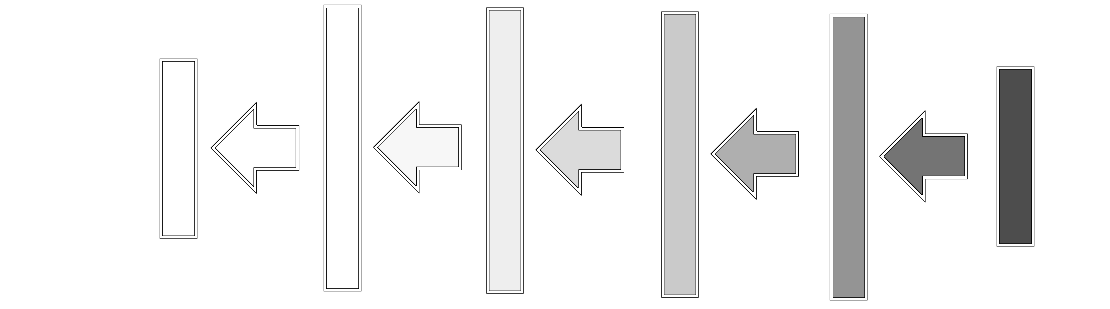
\includegraphics[width=0.7\linewidth]{images/4_vanishing_gradient}
\caption[]{Der \textit{Vanishing Gradient}-Effekt beschreibt bei der Rückpropagierung das abklingende Fehlersignal von Output- hin zu Input-Layer}
\label{fig:4_vanishing_gradient}
\end{figure}

Deutlich wird der Effekt bei der Betrachtung der Formel \ref{eq:vanishgrad1} für das zurück propagierte Fehlersignal $\delta_{message}^l$ im Layer $l$, in der aus Kapitel  \ref{ch:cnn_back} bekannten $\delta_{message}$-Notation.
\begin{equation}
\label{eq:vanishgrad1} 
\delta_{message}^{l} = (W^{l})^T (\delta_{message}^{l+1} \circ \phi'(z^l))
\end{equation}
Setzt man klassische Aktivierungsfunktionen wie $sig(\cdot)$ oder $tanh(\cdot)$ ein (siehe Kapitel \ref{ch:aktivierungsfunktonen}), gilt $\phi'(z^l) <= 1 $. Dies führt zwangsläufig zu einem abklingenden Fehlersignal (\textit{Vanishing Gradient}). Man könnte argumentieren, dass dies durch ein großes $W^l$, sodass $ (W^{l})^T (\delta_{message}^{l+1} \circ \phi'(z^l)) >= 1$, verhindert werden könnte. Dem ist nicht der Fall, da gleichzeitig $z^l = W^lx^l + b^l$ gilt und damit ein großes $W^l$ unweigerlich zu einem großen $z^l$ und damit zu einer kleineren Ableitung der Aktivierungsfunktion, welche ihr Maximum bei $0$ besitzt, führt. Ist zusätzlich zu einem großen $W^l$ der Schwellwert $b^l$ negativ, sodass $z^l \approx 0$, führt dies ebenso nicht zum Verschwinden des Effekts sondern zu einem, nicht weniger ungünstigen, \textit{Exploding Gradient}-Effekt \cite[vgl.][Kapitel 5]{Nielsen2015}). Selbst im linearen Fall ohne Aktivierungsfunktion tritt dieser Effekt auf, wenn die Gewichte jedes Neurons nicht die Norm $\|w\| \approx 1 $ besitzen.
 
Eine normalisierter Initialisierung der Gewichte wirkt diesem Effekt entgegen (vgl. \cite{Glorot2010}). Allerdings scheint erst die Verwendung der neuartigen ReLu-Aktivierungsfunktion (vgl. Kapitel \ref{ch:aktivierungsfunktonen}) den Effekt gänzlich zu unterdrücken und führt darüber hinaus zu oftmals er\-wünsch\-ten, dünnbesetzten (\textit{sparse}) Aktivierungen (vgl. \cite{Glorot2011}). Der Nachteil von ReLu-Neuronen ist allerdings, dass diese bei zu großen Lernraten und damit zu großen Änderungen der Gewichte unwiderruflich sterben (\textit{Dying ReLu}) und somit Teile des Netzes auslöschen können (vgl. \cite{Maas2013}).   


\begin{equation} 
	f(x) =  max(0,x) 
\end{equation}


\begin{figure}
\centering
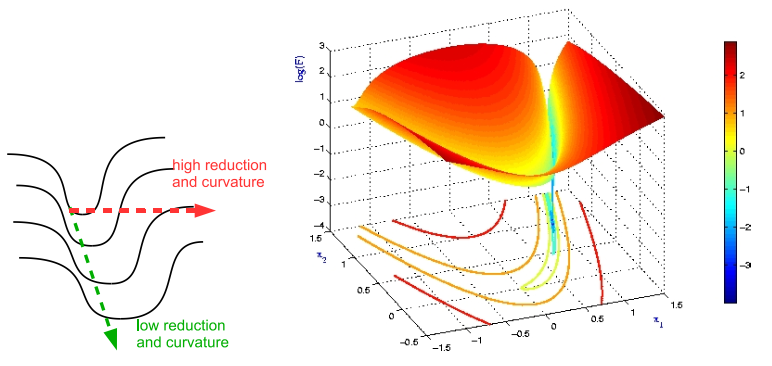
\includegraphics[width=0.5\linewidth]{images/4_pathological_curvature}
\caption[]{Pathological Curvature in der Rosenbrock-Funktion: $f(x,y = (1-x)^2 + 100(y -x^2)^2$ (vgl. \cite{Martens2010})}
\label{fig:4_pathological_curvature}
\end{figure}

Viele der in diesem Kapitel vorgestellten Methoden zielen auf den  \textit{Vanishing Gradient}-Effekt ab, welcher für viele Probleme im Deep-Learning verantwortlich ist. Darüber hinaus zeigt \cite{Martens2010} empirisch, dass die Schwierigkeiten im Deep-Learning auch auf eine ungünstige Fehlerlandschaft (\textit{Pathological Curvature}) zurückzuführen sind. Eine solche ist in Form der Rosenbrock-Funktion in Abbildung \ref{fig:4_pathological_curvature} dargestellt. 

Neben den benannten Problemen hinsichtlich der Fehlerfunktion, führt \textit{Overfitting} häufig ebenso zu schlechten Ergebnissen und entsprechende Regularisierungsmethoden werden benötigt.

\section{Vorverarbeitung}
Der Bereich Vorverarbeitung steht nicht unmittelbar in Zusammenhang mit Deep Learning, wird jedoch zwecks der Vollständigkeit, besonders in Verbindung zu CNNs, vorgestellt.
\cite{Becker1991} stellte bereits Anfang der 1990er Jahre fest, dass durch Dekorrelation der Trainingsdaten MLPs effizienter trainiert werden können. 
\cite{LeCun1998b} fassen die klassische Vorverarbeitung in linearen MLPs wie folgt zusammen:
\begin{itemize}
\item Mittelwertfreie Trainingsdaten verhindern eine steile Fehlerlandschaft. 
\item Die Normalisierung der Varianz unterschiedlicher Merkmale verhindert deren unterschiedliche Gewichtung.
\item Die Dekorrelation der Trainingsdaten führt zwar zu einer diagonalen Hesse-Matrix, allerdings zeigt der Gradient nicht in Richtung Minimum. Dies muss durch dedizierte Lernraten, entsprechend den Kehrwerten der Eigenwerte pro Gewicht, korrigiert werden.
\item Das Whitening der Daten führt zu einer kreisförmigen Fehlerlandschaft mit korrektem Gradienten.
\end{itemize}
Diese Hinweise gelten nur für lineare MLPs und somit quadratische Fehlerlandschaften. Die Fehlerlandschaft der hier verwendeten nicht-linearen MLPs kann jedoch lokal quadratisch approximiert werden (vgl. \cite{Hinton2015}).

Die genannten Techniken können allerdings nicht unmittelbar auf CNNs übertragen werden, da diese versuchen lokale Korrelationen an verschiedenen Orten im Eingaberaum zu extrahieren und die Dekorrelation hochdimensionaler Daten in großer Anzahl sehr rechenintensiv ist.
So zeigt sich bei der Verwendung von CNNs, dass die erfolgreichsten Architekturen lediglich den Mittelwert über die gesamten Trainingsdaten berechnen und diesen von jedem Pixel subtrahieren (vgl. \cite{Krizhevsky2012} und \cite{Simonyan2014}).
\cite{Kaparthy2014} kommen zu einem ähnlichen Schluss und beschreiben für CNNs lediglich die Zentrierung der Daten mittels globalen Mittelwert, alternativ pro Farbkanal oder Pixel, als nötige Vorverarbeitung. 

Teilweise werden für CNNs dennoch zwei weitere Techniken als Praxis beschrieben (vgl. \cite{Andrade2014} und \cite{Goodfellow_maxout_2013}) und deshalb im Folgenden kurz eingeführt.

\subsection{Kontrastnormalisierung}
Das Ziel der Kontrastnormalisierung ist es, unterschiedliche Trainingsbeispiele desselben Objekts in einen ähnlichen Kontrastbereich zu transformieren und so Helligkeitsunterschiede zu kompensieren (vgl. \cite{Zeiler2013b}). 

Die globale Kontrastnormalisierung (GCN) bearbeitet jedes Trainingsbeispiel einzeln und berechnet den Mittelwert und die Varianz über alle Merkmale beziehungsweise Pixel. Im Anschluss wird der Mittelwert subtrahiert und durch die Varianz geteilt \cite[vgl.][]{Sermanet2012}. 
Neben der GCN wird häufig auch die lokale Kontrastnormalisierung (LCN) angewandt. Diese nimmt pro Trainingsbeispiel als Eingabe jeweils nur kleine Umgebungen $k_h \times k_w$ und berechnet die Kontrastnormalisierung für diese Bereiche einzeln \cite[vgl.][]{Jarrett2009}.

\cite{Zeiler2013b} verwenden für Farbbilder den RGB-Raum und normalisieren jeden Kanal einzeln. Dies kann jedoch zu einer Verschiebung des Farbtons führen. Soll dies vermieden werden, wird für Farbbilder entweder der HSV-Raum vorgeschlagen, in welchen nur die Intensität $V$ normalisiert wird \cite[vgl.][S. 56]{Pink2011}. Oder es wird der YUV-Farbraum verwendet und die Normalisierung lediglich auf den Y-Kanal angewandt \cite[vgl.][]{Sermanet2012}.


\subsection{ZCA-Whitening}
Der Begriff \textit{Zero Component Analysis} (ZCA) beschreibt ein der \textit{Principle Component Analysis} (PCA) sehr ähnliches Verfahren (vgl. hierzu und im Folgenden \cite{Krizhevsky2009}). Es zielt darauf ab, die Eingangsdaten so zu dekorrelieren, sodass die Transformation so nahe wie möglich am Original ist. 

\begin{figure}
\centering
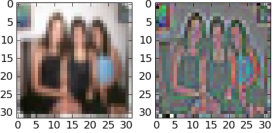
\includegraphics[width=0.5\linewidth]{images/4_ZCA}
\caption[]{Originales Bild (links) und ZCA-transformiertes Bild (rechts) (siehe. \cite{Krizhevsky2009})}
\label{fig:4_ZCA}
\end{figure}

Die Transformationsmatrix $W_{ZCA}$ ist in Gleichung \ref{eq:ZCA} angegeben, wobei die Kovarianzmatrix $C = X^TX$ ist. Der einzige Unterschied zum PCA-Whitening liegt darin, dass eine weitere Rotation zurück in den Bildraum durchgeführt wird. Dies ist möglich, da das Whitening der Daten auch nach einer Rotation mit einer orthogonalen Matrix erhalten bleibt.

\begin{equation}
\label{eq:ZCA} 
W_{ZCA} = C^{-\frac{1}{2}} = P(D+\epsilon)^{-\frac{1}{2}}P^T = PW_{PCA}
\end{equation}

Abbildung \ref{fig:4_ZCA} zeigt die Transformation für ein Beispiel.


\section{Initialisierung}
Die Initialisierung eines neuronalen Netzes ist äußerst wichtig, da die Gewichte ungleich Null sein müssen (\textit{Breaking the Symmetry}). Ansonsten berechnen alle Neuronen die gleiche Ausgabe und es ergeben sich somit die gleichen partiellen Ableitungen \cite[vgl.][S. 201]{Rojas1996}.
\cite{LeCun1989} initialisieren die Gewichte beispielsweise zufällig zwischen $-\frac{2.4}{fan_{in}}$ und $\frac{2.4}{fan_{in}}$, wobei $fan_{in}$ der Anzahl Eingangsneuronen entspricht. Das hat zum Ziel die Nichtlinearität mit Werten um Null zu versorgen und damit nicht zu sättigen (\textit{Vanishing Gradient}).
Das erfolgreiche Netz von \cite{Krizhevsky2012} verwendet beispielsweise die Standard-Initialisierung, eine einfache Normalverteilung mit $W \sim \mathcal{N} (0,0.01)$. Dies ist möglich, da als Aktivierungsfunktionen ReLu-Funktionen verwendet werden, welche nicht sättigen können. 

Daneben existieren im Deep Learning heute zwei Arten zur Initialisierung, welche im Folgenden aufgeführt sind. 

\subsection{Normalisierte Fehlerpropagierung}
\begin{figure}
\centering
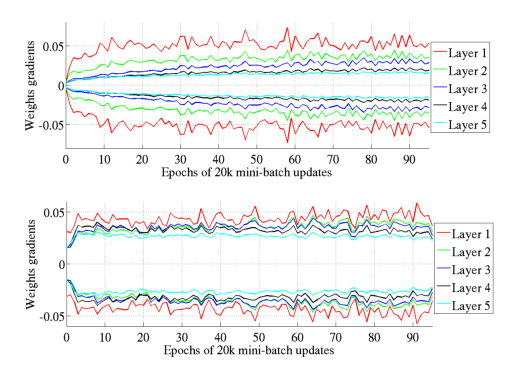
\includegraphics[width=0.7\linewidth]{images/4_xavier_init}
\caption[]{Vergleich der Varianz der Gradienten im Laufe des Trainings (Standard-Initialisierung (oben) und Xavier-Initialisierung (unten)): \textit{Layer 1} entspricht dem Output-Layer mit der größten Varianz im Gradient (siehe \cite{Glorot2010})}
\label{fig:4_xavier_init}
\end{figure}
Stellvertretend für eine derartige Initialisierung der Gewichte, sodass die Varianz des Signals sowohl bei der Berechnung der Ausgabe (\textit{Forward Pass}), als auch bei der Rückpropagierung des Fehlers (\textit{Backward Pass}) gleich groß bleibt  \cite[vgl. z.B.][S. 199 ff.]{Rojas1996}, steht heute die sogenannte \textit{Xavier-Initialization}. Dies führt dazu, dass die Varianz im Gradienten in jeder Schicht in etwa gleich groß ist, was aus Abbildung \ref{fig:4_xavier_init} zu entnehmen ist (vgl. hierzu und im Folgenden \cite{Glorot2010}).
Die \textit{Xavier-Initialization} kombiniert beide Aspekte und initialisiert die Gewichte in der Art, dass die Varianz des Signals von Schicht zu Schicht sowohl im \textit{Forward Pass} als auch im \textit{Backward Pass} erhalten bleibt. Dies wird durch Formel \ref{eq:xavier} erreicht, was letztlich der Anwendung der Varianz-Formel für Gleichverteilung mit $Var(W) = \frac{2}{fan_{in}  + fan_{out}}$ entspricht.

\begin{equation}
\label{eq:xavier} 
W \sim \mathcal{U} [-\frac{\sqrt{6}}{\sqrt{fan_{in}  + fan_{out}}}, \frac{\sqrt{6}}{\sqrt{fan_{in}  + fan_{out}}}]
\end{equation}

Für den Fall, dass ReLu-Funktionen eingesetzt werden, verallgemeinern \cite{He2015} diese Formel insofern, dass eine lineare Approximation um Null für diese und davon abgeleitete Aktivierungsfunktionen nicht mehr gültig ist. Formel \ref{eq:xavier2} entspricht der Verallgemeinerung für Funktionen dieser Art. 

\begin{equation}
\label{eq:xavier2} 
W \sim \mathcal{N} (0,\sqrt{\frac{2}{fan_{out}}})
\end{equation}

Mit der Xavier-Initialisierung werden in Folge häufig bessere Ergebnisse erreicht, als mit der Standard-Initialisierung (\textit{Random Initialization}) in Verbindung mit Informationen über die Krümmung (Approximation der Hesse-Matrix - siehe. Kapitel \ref{ch:2norder}) (vgl. \cite{Chapelle11} und \cite{Glorot2010}).
Für Convolutional Neural Networks berechnen sich \textit{$fan_{in}$} und \textit{$fan_{out}$} durch Multiplikation der Filtergröße mit der Anzahl \textit{Input-Maps} respektive \textit{Feature-Maps} $c$: $k_w \cdot k_h \cdot c$ \cite[vgl.][]{He2015}.


\subsection{Unüberwachtes Vortraining}
Dieses Kapitel weicht die in Kapitel \ref{ch:Einleitung} gemachte Einschränkung auf das klassische überwachte, neuronale Lernmodell insofern auf, als dass ein un\-über\-wach\-tes Lernverfahren vorgestellt wird. Dieses Vorgehen dient jedoch zum einen dem höheren Ziel, das überwachte Verfahren durch eine bessere Initialisierung der Gewichte besser zu konditionieren und in der Performanz zu verbessern. Zum anderen wird sich zeigen, dass es sich bei genauerer Betrachtung nicht um ein klassisches un\-über\-wach\-tes Lernverfahren handelt: Es wird lediglich ein un\-über\-wach\-tes Problem als überwachtes Problem angesehen. 
Dies lässt sich am einfachen Beispiel eines nichtlinearen Autoencoders verdeutlichen \cite[vgl. hierzu und im Folgenden][]{Masci2011}. Der Encoder in Formel \ref{eq:autoenc1} nimmt als Eingabe einen Vektor $x$ und berechnet einen Code $h$.
  
\begin{equation}
\label{eq:autoenc1} 
h = \phi(Wx + b)
\end{equation}

Dieser Code wird im zweiten Schritt durch den Decoder in Formel \ref{eq:autoenc2} dekodiert und so die Ausgabe berechnet. Das Ziel des Autoencoders ist es den Fehler zwischen Eingabe und Rekonstruktion, wie z.B. $MSE = \mathbb{E} [ (x - y)^2 ]$, durch Anpassen der Gewichte $ \theta={W,b} $, wobei $W' = W^T$ (\textit{Tied Weights}), zu minimieren.
 
\begin{equation}
\label{eq:autoenc2} 
y = \phi(W'h + b')
\end{equation}

Der Autoencoder prädiziert folglich die Eingabe selbst und lernt die sogenannte Identität (\textit{Identity Mapping}).
Die Ideen von \cite{Hinton2006}, die gleichzeitig auch den Beginn der Renaissance von Deep Learning darstellen, beschreiben ein Verfahren große Netzwerke mit vielen Schichten schichtweise \textit{greedy} mit beschränkten Boltzmann Maschinen (RBMs) zu trainieren (vgl. \cite{Bengio2007}). Das bedeutet, dass jede Schicht als Eingabe die Ausgabe der vorherigen Schicht erhält und versucht, diese wiederum zu prädizieren (vgl. \cite{Ranzato2006}). Dies wirkt ähnlich wie ein Regularisierer und initialisiert die Gewichte hinsichtlich der Optimierung und Generalisierung in einer besseren Ausgangssituation \cite[vgl.][]{Erhan2010}. Hiervon profitieren besonders große MLPs, welche bis dato aufgrund des \textit{Vanishing-Gradient}-Effekts als schwer zu trainieren galten. 

Eine wichtige Weiterentwicklung des Konzepts sind sogenannte \textit{Denoising Autoencoder} (DAs) beziehungsweise \textit{Stacked Denoising Autoencoder} (SDA), welche versuchen die Eingabe $ x $ ausgehend von einer korrumpierten Version $ \hat{x} $ zu prädizieren. Dies erlaubt das Erlernen robuster Merkmale und kann als diskriminative Alternative zum generativen stochastischen RBM-Modell gesehen werden (vgl. \cite{Vincent2008}). 

Convolutional Neural Networks wie das \textit{LeNet 5} von \cite{LeCun1998} können aufgrund ihrer besonderen Struktur dennoch trainiert werden. Trotzdem ist es auch bei CNNs schwierig die ersten Schichten zu trainieren, da die hinteren Schichten generell schneller unscheinbares \textit{Overfitting} mit entsprechend kleinem Gradienten aufweisen (vgl. \cite{Erhan2010}). Der erste Versuch un\-über\-wach\-tes Vortraining auf CNNs anzuwenden stammt von \cite{Ranzato2006}. Hier wird die erste Schicht eines veränderten \textit{LeNet 5} mittels Vortraining initialisiert, was den Fehler auf dem MNIST-Datensatz\footnote{Der MNIST-Datensatz handgeschriebener Ziffern besteht aus 60,000 Trainingsbeispielen und 10,000 Testbeispielen. Es stellt eine Untermenge des größeren NIST-Datensatzes dar. Die Bilder sind $28 \times 28$ und die Ziffern zentriert (\url{http://yann.lecun.com/exdb/mnist/} (26.08.2015)).} von $0.7 \%$ auf $0.6 \%$ verringert. Das Vortraining der $5 \times 5$-Filter geschieht mit zufällig gewählten $5 \times 5$-Bildausschnitten auf der Basis von RBMs.


\subsubsection{Convolutional Autoencoder}
\label{ch:autoenc}
Es existieren verschiedenste Architekturvorschläge für Autoencoder und RBMs zum Vortraining von CNNs. Die Grundlage hierfür ist meist die Extraktion den Filter entsprechend großer Bildausschnitte und das Trainieren gewohnter Modelle (vgl. \cite{Desjardins2008}, \cite{Ranzato2007} oder \cite{Lee2009}).  
Im Folgenden wird der Convolutional Autoencoder von \cite{Masci2011} vorgestellt, da dieser auf Faltungen basiert und, wie Abbildung \ref{fig:4_mascii} zeigt, die gewünschten translationsinvarianten Filter erzeugt. Die vorgestellte Variante verbessert im Rahmen der Experimente von \cite{Masci2011} den Testfehler auf dem MNIST-Datensatz von $0.79 \%$ auf $0.71 \%$.

\begin{figure}
\centering
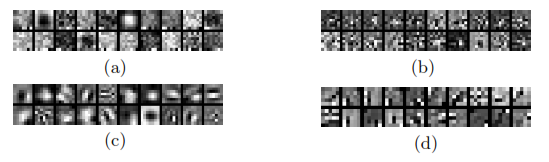
\includegraphics[width=0.7\linewidth]{images/4_mascii}
\caption[]{Filter der ersten Schicht eines Convolutional Autoencoders (a) Kein Max-Pooling, 0 \% Rauschen, (b) Kein Max-Pooling, 50 \% Rauschen, (c) Max-Pooling $2 \times 2$, (d) Max-Pooling $2 \times 2$, 30 \% Rauschen (siehe \cite{Masci2011})}
\label{fig:4_mascii}
\end{figure}

Die Architektur des vorgestellten Convolutional Autoencoders besteht aus einem Convolution-Layer sowie einem nachgeschalteten Pooling-Layer. Das bedeutet, dass sich der gesamte Autoencoder letztendlich aus zwei hintereinander ausgeführte Layern dieser Art zusammensetzt.

Gleichung \ref{eq:cautoenc1} zeigt die Berechnung des Codes $h_i$ der $i$-ten \textit{Feature-Map}. Dieser wird wie in gewöhnlichen CNNs durch Faltung mit Randbehandlung \textit{valid} berechnet. 

\begin{equation}
\label{eq:cautoenc1} 
h_i = \phi(\sum_{j=0}^{m}  x_{j} \ast W_{ij} + b_i)
\end{equation}

Der Decoder berechnet die Funktion \ref{eq:cautoenc2}, wobei ähnlich dem \textit{Backward Pass} im Backpropagation die Filtermaske über beide Seiten geflippt beziehungsweise um $180^\circ$ gedreht und die Randbehandlung \textit{full} verwendet wird. Die Dekodierung ist beeinflusst von gewöhnlichen Autoencodern mit \textit{Tied Weights}, bei denen als Dekodierungsfunktion ebenfalls die transponierte Gewichtsmatrix des \textit{Forward Pass} verwendet wird.

\begin{equation}
\label{eq:cautoenc2} 
y_j = \phi(\sum_{i=0}^{n} h_{i} \ast rot180(W_{ij}) + c_j)
\end{equation}

Der Gradient für den Autoencoder berechnet sich mit Formel \ref{eq:cautoenc3}. Diese setzt sich, wie der Autoencoder, aus zwei Teilen zusammen. Der erste Teil wird für den Encoder, der zweite für den Decoder benötigt. Im Unterschied zur Berechnung des Gradienten beim CNN wird anstatt $\delta y$ der Code $h$ der Flip-Operation unterzogen. Dies tritt auf, da der \textit{Backward Pass} dem eigentlichen \textit{Forward Pass} entspricht.\footnote{Im Unterschied zur von \cite{Masci2011} beschriebenen Berechnung wird in Konsequenz auch auf die Flip-Operation von $\delta h$ nicht verzichtet und der Gradient am Ende gesamtheitlich geflippt. Der Gradient für den Encoder wird damit äquivalent zu dem in einem CNN berechnet. In Kapitel \ref{ch:debug} wird die Richtigkeit dieser Änderung überprüft.}
Eine zusätzliche Besonderheit besteht in Zusammenhang mit der Randbehandlung \textit{valid}. Um den Code $rot180(h)$ mit dem räumlich größeren $\delta y$ der Ausgabe zu falten, muss dieser doppelt mit Nullen erweitert werden (Padding). Zum einen um die gleiche Größe wie die Ausgabe zu erhalten und zum anderen um die Faltung zu ermöglichen.

\begin{equation}
\label{eq:cautoenc3} 
\frac{\partial J(W,b,c)}{\partial W_{ij}^l} = \frac{1}{M} \sum_{m=1}^{M} rot180(x_{mj}^l \ast  rot180(\delta h_{mi}^l) + rot180(h_{mi}^l) \ast \delta y_{mj}^l)   
\end{equation}

Analog zum bekannten Convolution-Layer wird über alle Trainingsbeispiele $M$ gemittelt und die beiden Schwellwerte $b$ und $c$ berechnen sich aus der Summe der zugehörigen Deltas $\delta y$ und $\delta h$, wie in Gleichung \ref{eq:cautoenc4} und \ref{eq:cautoenc5} dargestellt ist.

\begin{equation}
\label{eq:cautoenc4} 
\frac{\partial J(W,b,c)}{\partial b_{i}^l} = \frac{1}{M} \sum_{m=1}^{M} \sum_{u=0}^{k_w} \sum_{v=0}^{k_w} \delta h_{miuv}^{l} 
\end{equation}


\begin{equation}
\label{eq:cautoenc5} 
\frac{\partial J(W,b,c)}{\partial c_{j}^l} = \frac{1}{M} \sum_{m=1}^{M} \sum_{u=0}^{k_w} \sum_{v=0}^{k_w} \delta y_{miuv}^{l} 
\end{equation}


Weiterentwicklungen wie die \textit{Tiled CNNs} versuchen weitere Invarianzen, wie beispielsweise die Rotationsinvarianz, zu lernen (vgl. \cite{Quoc2010}).
Einer der größten Autoencoder, der \textit{Google Autoencoder}, bedient sich ebenfalls der lokalen rezeptiven Felder, verzichtet allerdings auf \textit{Parameter Sharing}, um verschiedene Invarianzen zu lernen (vgl. \cite{LeRanzato2012}). Eine Schicht dieser Architektur ist in Abbildung \ref{fig:4_ranzato} abgebildet.

\begin{figure}
\centering
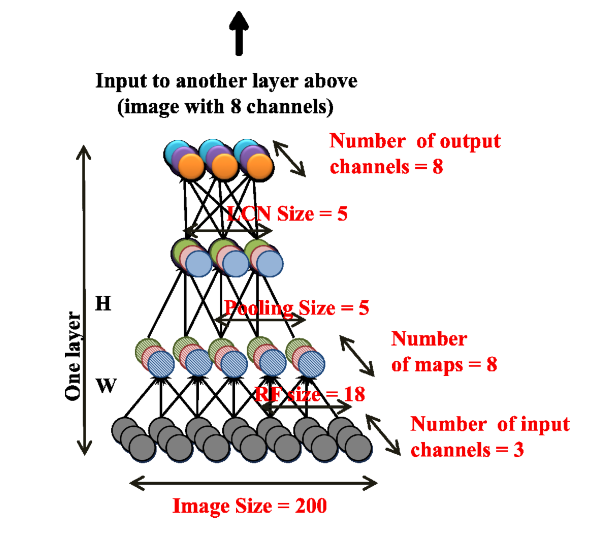
\includegraphics[width=0.5\linewidth]{images/4_ranzato}
\caption[]{Autoencoder mit lokalen rezeptiven Feldern aber ohne \textit{Parameter Sharing} (siehe \cite{LeRanzato2012})}
\label{fig:4_ranzato}
\end{figure}


Auch wenn das Verwenden von un\-über\-wach\-tem Vortraining für die ersten Schichten eines CNNs passend erscheinen mag, führt es nicht zu einer solchen Verbesserung der Ergebnisse wie bei tiefen MLPs (DNNs) (vgl. \cite{Hamid2013}). 
Durch die Entwicklung neuer Aktivierungsfunktionen wie ReLu und raffinierter Initialisierung rückt das Thema somit in solche Bereiche, in denen wenig gelabelte Trainingsdaten zur Verfügung stehen, um das CNN vollständig überwacht zu trainieren (vgl. \cite{Masci2011} und \cite{LeRanzato2012}). Darüber hinaus können auch verbesserte Optimierungsverfahren das un\-über\-wach\-te Vortraining hinsichtlich einer besseren Initialisierung ersetzen (vgl. \cite{Martens2010} und \cite{Sutskever2013}). 

Eine neue Herangehensweise ist es, bereits trainierte CNNs für andere Probleme zu übernehmen, was als sogenanntes Transferlernen bezeichnet wird (vgl. \cite{Wagner2013}). So liefert zum Beispiel die 7. Schicht des \textit{AlexNet} von \cite{Krizhevsky2012} bereits sehr gute Bildbeschreibungen (vgl. \cite{Bell2015} und \cite{Kaparthy2014}).


\section{Gradientenabstieg}
\label{ch:gradient}
\begin{figure}
\centering
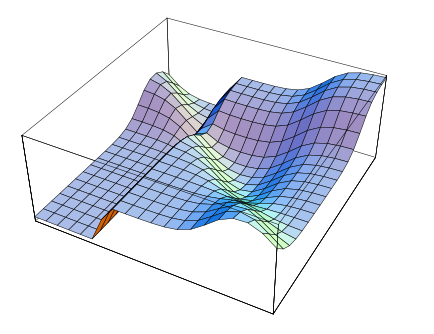
\includegraphics[width=0.5\linewidth]{images/4_Gradient2}
\caption[]{Fehlerfunktion beziehungsweise Zielfunktion im Gewichtsraum mit lokalem Minimum \cite[siehe][S. 155]{Rojas1996} }%\cite[siehe][Kap. 5, S. 17]{Duda2001}}
\label{fig:4_Gradient}
\end{figure}
Dieses Kapitel behandelt verschiedene Methoden zur Verbesserung des Gradientenabstiegs. Diese können das Training erheblich beschleunigen, da es sich im Allgemeinen im Deep Learning um nicht-konvexe Fehlerlandschaften wie in Abbildung \ref{fig:4_Gradient} handelt.

Die Grundlage für das effiziente Lernen mit vielen Trainingsdaten ist der sogenannte stochastische Gradientenabstieg (SGD) (vgl. hierzu und im Folgenden \cite{Bottou1998}). Hierbei geht es um die Frage, was die erwartete durchschnittliche Richtung des Gradienten ist. Durch die Einführung des MSE-Fehlermaßes ist der Ansatz des SGD bereits gegeben. So entspricht die MSE-Fehlerfunktion dem Erwartungswert der einzelnen Fehlerquadrate. Wie in Gleichung \ref{eq:sgd_mse} zu sehen ist, entspricht analog dazu der Erwartungswert der einzelnen Gradienten dem Gradient der Fehlerfunktion.

\begin{equation}
\label{eq:sgd_mse} 
\nabla J(W,b) =  \mathbb{E}[\nabla (f(x_i) - y_i)^2] = \frac{1}{N}\sum_{i}^{N} \nabla (f(x_i) - y_i)^2
\end{equation}

Für eine allgemeine Fehlerfunktion $e(x)$ gilt: Nimmt man an Stelle der gesamten Trainingsmenge $N$ (Batch) einzelne Trainingsbeispiele $i$ (Online) oder eine Teilmenge $M$ (Averaged SGD), so ergibt sich Formel \ref{eq:sgd} für den Gradientenabstieg mit Lernrate beziehungsweise Schrittweite $\eta$. Der Gradient zeigt somit in Richtung des Durchschnitts und damit in Richtung des Erwartungswerts. 

Neben einer effizienteren Berechnung des Gradientenabstiegs, liefert SGD eine Zufallskomponente (\textit{Randomization}) \cite[vgl. hierzu und im Folgenden][]{Bengio2012}. Diese kann zu beschleunigter Konvergenz führen, da durch variierende (\textit{noisy}) Gewichtsupdates ein größeres Gebiet untersucht werden kann. Außerdem erlaubt SGD Training ohne unmittelbarem Zugriff auf die gesamte Trainingsmenge. Üblicherweise werden die für die Berechnung entnommenen Teilmengen als \textit{Mini-Batch} bezeichnet.

\begin{equation}
\label{eq:sgd} 
W_{t+1} = W_t - \eta \frac{1}{M} \sum_{i=1}^{M} \nabla e(x_i)
\end{equation}

SGD bildet die Grundlage für viele Erweiterungen und stellt so die erste Optimierung des Gradientenabstiegs dar. 
Um die Formeln zu vereinfachen, wird im Folgenden auf die sonst obligatorische Mittelung des Gradienten verzichtet. An den entsprechenden Stellen wird darauf hingewiesen, ob es sich um die Erweiterung für den Online-/Mini-Batch-Modus oder um den klassischen Batch-Modus, welcher für Deep Learning in Verbindung mit vielen Trainingsdaten unpraktikabel ist, handelt. 

\subsubsection{Lernrate und Mini-Batch-Größe}

Wird der klassische Gradientenabstieg ohne Optimierungen verwendet, ist es besonders wichtig $\eta$ richtig zu wählen. Aufgrund des \textit{Vanishing Gradient}-Effekts sollte die Lernrate in den letzten Schichten kleiner gewählt werden. Außerdem ist darauf zu achten, dass die Lernrate durch \textit{Parameter Sharing} proportional zur Wurzel der Verbindungen ist, die sich ein Gewicht teilen. Letzteres ist gerade bei CNNs zu beachten, um eine unnötig schlechte Konditionierung der Fehlerlandschaft zu vermeiden (vgl. \cite{LeCun1998b}).

Die Bestimmung der Mini-Batch-Größe $M$ erlaubt es zwischen Online- und Batch-Training zu interpolieren. Dies ist wichtig, da die richtige Wahl der Größe von den Trainingsdaten abhängt und nicht allgemein vorhergesagt werden kann. So kann beispielsweise Online-Training in vielen Situationen schneller sein als Batch-Training  \cite[vgl.][]{Wilson2003}. Als Stellgröße kann der Grad an Redundanz in den Trainingsdaten dienen. Mit steigender Redundanz sollten die Batches entsprechend kleiner gewählt werden, um nicht unnötig Rechenzeit zu verbrauchen. \cite{Bengio2012} nennt $M = 32$ einen guten Standardwert.

\subsection{Momentum}
Eine der ersten erfolgreichen Erweiterungen für iterative Verfahren ist die sogenannte Momentum Methode von \cite{Polyak1964}.
Die Momentum-Methode ist durch die Physik motiviert, dadurch dass dem Gradienten eine potentielle Energie zugewiesen wird. Dies erlaubt es in gleichbleibender Richtung des Gradienten Geschwindigkeit aufzunehmen. Dies führt letztendlich dazu, dass in flachen Regionen der Fehlerlandschaft größere und in unwegsamen Bereichen kleinere Schrittweiten effektiv ausgeführt werden (vgl. \cite{LeCun1998b}).
Dies wird durch das Hinzufügen eines weiteren Terms in das Gewichtsupdate erzielt. Wie Formeln \ref{eq:momentum} und \ref{eq:momentum1} zeigen, bildet die Momentum-Methode einen gewichteten Durchschnitt der vergangenen Gradienten der Gewichte. 
 
\begin{equation}
\label{eq:momentum} 
\Delta W_t = \mu \Delta W_{t-1} - \eta \nabla J(W_t,b_t)
\end{equation} 
 
\begin{equation}
\label{eq:momentum1} 
W_{t+1} = W_t + \Delta W_t
\end{equation}
Typische Werte für die Momentum-Rate $\mu$ sind Werte größer $0.9$. Diese sind allerdings abhängig vom Lernproblem und können nicht allgemein formuliert werden (vgl. \cite{Kaparthy2014}). Die Momentum-Methode ist eine sehr einfache Optimierung für SGD und findet in erfolgreichen Netzen häufig Anwendung (vgl. \cite{Krizhevsky2012}).

\subsubsection{Nesterov-Methode}
Die Nesterov-Methode (NAG) ist eine verbesserte Momentum-Methode, die von \cite{Nesterov1983} beeinflusst ist \cite[vgl. hierzu und im Folgenden][]{Sutskever2013b}. Diese Methode führt zunächst den über die vergangenen Perioden gewichteten Momentum-Term aus und berechnet dann den Gradient an dieser Stelle. Die Methode fungiert somit als eine Art Ausblick auf die zukünftige Fehlerlandschaft. Der eigentliche Gradient ergibt sich schließlich aus Ausblick und Korrektur, wie Abbildung \ref{fig:4_nesterov} zeigt.
\begin{figure}
\centering
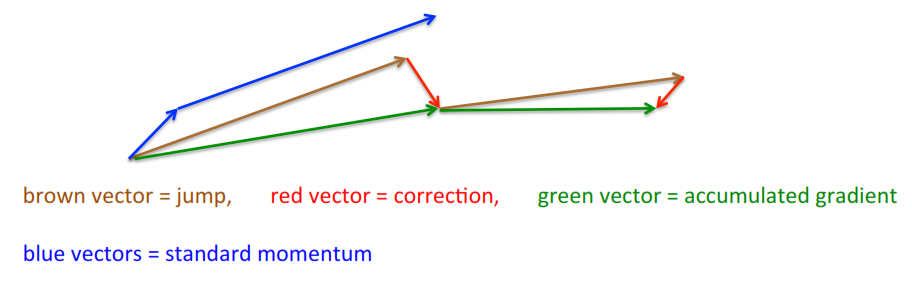
\includegraphics[width=0.7\linewidth]{images/4_nesterov}
\caption[]{Das effektivere Nesterov-Momentum korrigiert Fehler im Nachhinein\cite[siehe][]{Hinton2015} }%\cite[siehe][Kap. 5, S. 17]{Duda2001}}
\label{fig:4_nesterov}
\end{figure}

Da diese Ausführung die Reihenfolge des üblichen Trainings beeinflussen würde, wird die Methode derart umgeschrieben, dass die aktuellen Gewichte immer dem Ausblick entsprechen. Daraus ergeben sich die Regeln \ref{eq:nesterov1} und \ref{eq:nesterov2} für die Aktualisierung der Gewichte (vgl. \cite{Kaparthy2014}).


\begin{equation}
\label{eq:nesterov1} 
\Delta W_t = \mu \Delta W_{t-1} - \eta  \nabla J(W_t,b_t)
\end{equation}
\begin{equation}
\label{eq:nesterov2} 
W_{t+1} = W_t + (-\mu \Delta W_{t-1} ) + (1 + \mu) \Delta W_t
\end{equation}

Die beschriebene Methode ist nach \cite{Sutskever2013} robuster hinsichtlich der Momentum-Rate und lässt höhere Raten zwischen $0.9$ und $0.99$ zu. 

\subsection{Adaptive Lernrate}
\label{ch:2norder}
Ein allgemeines Problem in Verbindung von Gradientenabstieg und dem Training im Deep Learning ist der \textit{Vanishing Gradient}-Effekt nach \cite{Hochreiter1991}. Ein Algorithmus der direkt auf diesen Effekt abzielt, ist der sogenannte Resilient Propagation, auch Rprop genannt (vgl. \cite{Riedmiller1992} und \cite{Igel2000}). Rprop weist jedem Gewicht eine eigene Lernrate zu und verzichtet verwendet nur das Vorzeichen des Gradienten. Die grundlegende Arbeitsweise sieht vor, bei gleichbleibendem Vorzeichen der partiellen Ableitung eines Gewichts die zugehörige Lernrate zu erhöhen. Tritt ein Vorzeichenwechsel auf, so liegt es nahe, dass in der Richtung dieser Ableitung eine Senke übersprungen wurde und die Lernrate wird reduziert. Rprop ist nach \cite{Hinton2015} äquivalent zum Gradientenabstieg im Batch-Modus, wenn bei letzterem durch die Länge des Gradient geteilt wird.
Hier liegt ein fundamentales Problem hinsichtlich Deep Learning: Um die Länge des Gradienten korrekt zu schätzen, bedarf es der gesamten Trainingsmenge, was die Verwendung von SGD ausschließt. Somit ist Rprop nur für Batch-Training geeignet (vgl. \cite{Hinton2015}).



Der bekannte Newton-Algorithmus für Optimierung in Gleichung \ref{eq:hessianstep} multipliziert nicht mit einer globalen Lernrate, sondern mit der Inversen der Hesse-Matrix. Unter bestimmten Annahmen, wie etwa einer quadratischen Zielfunktion, erreicht dieser Algorithmus innerhalb eines Schrittes das Minimum, was als Newton-Schritt bezeichnet wird (vgl. \cite{Bottou1998}).

\begin{equation}
\label{eq:hessianstep} 
W_{t+1} = W_t - H_t^{-1} \nabla J(W_t,b_t)
\end{equation}

Die Hesse-Matrix ist im Allgemeinen sehr teuer zu berechnen, da jede partielle Ableitung der $N$ Gewichte nochmals abgeleitet werden müsste. Dies führt auf eine $N \times N $-Matrix, welche in neuronalen Netzen nicht effizient zu berechnen ist und deshalb approximiert werden muss \cite[vgl.][]{LeCun1998b}. 

Algorithmen mit sogenannter adaptiver Lernrate gehen so vor, dass sie lediglich die Diagonale der Hesse-Matrix $diag(H)$ approximieren. Dies führt zu eigenen Lernraten pro Gewicht, welche idealerweise den echten Eigenwerten der Hesse-Matrix entsprechen \cite[vgl.][]{LeCun1998b}. Adaptive Lernraten erlauben es, Schrittweiten in Gegenden schwacher Krümmung zu erhöhen und entsprechend in anderen zu verkürzen. Dieser Mechanismus wirkt damit ebenso unmittelbar dem \textit{Vanishing Gradient}-Effekt entgegen, da kleiner werdende Gradienten zu den ersten Schichten hin skaliert werden \cite[vgl.][]{Martens2010}. 
Problematisch bei der Verwendung der Hesse-Matrix für nicht-konvexe Probleme sind negative Eigenwerte an lokalen Maxima oder gemischt positive und negative Eigenwerte an Sattelpunkten, die zu einer falschen Richtung des Gradienten führen \cite[vgl.][]{Dauphin14}. Aus diesem Grund ist es notwendig, eine Methode mit entsprechender Vorkonditionierung zu verwenden \cite[vgl.][]{Dauphin2015}.


\subsubsection{Stochastischer Levenberg-Marquardt}
Der bekannte stochastische Levenberg-Marquardt-Algorithmus (LMA) von \cite{LeCun1998b} ist ein Algorithmus im Bereich Neuronale Netze und SGD, der versucht die $diag(H)$ zu approximieren. Hierzu sind allerdings zwei weitere Approximationen notwendig. So wird die Gauß-Newton Approximation zur Vermeidung negativer Eigenwerte, wie im klassischen LMA-Algorithmus, angewandt und die $diag(H)$ nur auf einer kleinen Teilmenge der Trainingsdaten (Mini-Batch) berechnet. Darüber hinaus wird die Berechnung nur einmal pro Epoche durchgeführt. Die Kosten entsprechen denen eines normalen \textit{Forward Pass} sowie einem angepassten \textit{Backward Pass}, der zur Rückpropagierung der zweiten Ableitungen dient, und sind somit zu vernachlässigen. 
Neben der Kompensation des \textit{Vanishing-Gradient}-Effekts durch adaptive Lernraten, kompensiert der stochastische LMA den Effekt der schlechten Konditionierung der Fehlerlandschaft durch \textit{Parameter Sharing} \cite[vgl.][]{LeCun1998b}.
Die neue Lernrate pro Gewicht $i$ ergibt sich mit Formel \ref{eq:lma}.

\begin{equation}
\label{eq:lma} 
\eta_{i} = \frac{\eta}{\mu + H_{ii}}
\end{equation}

Wie im klassischen LMA wird ein Dämpfungsfaktor $\mu$ verwendet, um zu verhindern, dass die Schrittweite zu groß wird. Dieser Faktor kann auch als Vorannahme gesehen werden, die angibt, dass sich das Gewicht nicht ändern soll, wenn die Krümmung entsprechend klein wird (vgl. \cite{Martens2010}). Im \textit{LeNet 5} wird $\mu = 0.02$ verwendet.


\subsubsection{Equilibrium SGD}
Eine Verbesserung zum stochastischen LMA ist die von \cite{Dauphin2015} beschriebene Equilibrium-Methode, welche die Matrix $D^{Eq} = \sqrt{diag(H^2)})$ berechnet. Diese Vorkonditionierung bietet einige Vorteile hinsichtlich der Behandlung der genannten indefiniten Hesse-Matrizen, die durch Sattelpunkten innerhalb der Fehlerlandschaft von MLPs auftreten. Darüber hinaus kann diese Methode effizient durch den Zusammenhang in Formel \ref{eq:equi} mit $v \sim \mathcal{N} (0,1)$, beispielsweise mit dem $R\{\cdot\}$-Operator (vgl. \cite{Pearlmutter1994}), berechnet werden. 

\begin{equation}
\label{eq:equi} 
D^{Eq} = diag(H^2) = E[(Hv)^2]
\end{equation}

Im Unterschied zum stochastischen LMA bildet die Equilibrium-Methode, wie Formel \ref{eq:equi1} zeigt, einen  \textit{Root Mean Square}-Durchschnitt (RMS) über die vergangenen Perioden. \cite{Dauphin2015} schlagen eine Neuberechnung von $D^{eq}$ nach jeweils 20 Iterationen und $\mu \in [10^{-4},10^{-6}]$ vor.

\begin{equation}
\label{eq:equi1} 
D^{eq}_{t+1} = \rho D^{eq}_{t} + (1 - \rho) (Hv)^2
\end{equation}

Damit ergibt sich die in Formel \ref{eq:equi2} gezeigte effektive Lernrate, welche ebenfalls einen Dämpfungsfaktor $\mu$ zur Vermeidung großer Schrittweiten beinhaltet.

\begin{equation}
\label{eq:equi2} 
\eta_{i} = \frac{\eta}{\mu + \sqrt{D^{eq}_{ii}}}
\end{equation}

\subsubsection{RMSprop}
Der RMSprop-Algorithmus stammt von \cite{Hinton2015} und kombiniert zwei Ideen. Einerseits die Idee des Rprop nur auf das Vorzeichen des Gradienten zu achten, indem er den \textit{Root Mean Square}-Durchschnitt (RMS) der partiellen Ableitungen über mehrere Zeitschritte berechnet. Andererseits wird das Hauptproblem von AdaGrad der stetig kleiner werdenden effektiven Lernraten dadurch vermieden \cite[vgl.][Kap. 8.4.1, S. 257]{Bengio2015}. Die Formel \ref{eq:rmsprop1} beschreibt die Berechnung des RMS. Die effektive Lernrate berechnet sich mit der Formel \ref{eq:rmsprop2}, wobei ebenfalls ein Dämpfungsfaktor $\mu$ verwendet wird. Der Parameter $\rho$ gibt an mit welcher Rate der exponentiell geglättete Mittelwert abnimmt. \cite{Dauphin2015} schlagen $\mu = 10^{-2}$ und $\rho = 0.9$ als robuste Werte vor.

\begin{equation}
\label{eq:rmsprop1} 
\hat{H}_{t+1} = \rho \hat{H}_{t} + (1 - \rho) \nabla J(W_t,b_t)^2
\end{equation}


\begin{equation}
\label{eq:rmsprop2} 
\eta_{i} = \frac{\eta}{\mu + \sqrt{\hat{H}_{ii}}}
\end{equation}

Eine sehr interessante Eigenschaft von RMSprop ist die Fähigkeit zur Approximation der Equilibrium-Matrix $D^{Eq} = \sqrt{diag(H^2)})$ (vgl. \cite{Dauphin2015}). RMSprop stellt eine sehr effektive und praktische Optimierung dar, welche dazu einfach zu implementieren ist. Dies macht diese derzeit sehr beliebt (vgl. \cite{Bengio2015}).

\subsubsection{AdaDelta}
AdaDelta ist ein von \cite{Zeiler2012} entwickeltes Verfahren, welches ebenfalls das Problem der immer kleiner werdenden Lernrate von AdaGrad adressiert (vgl. \cite{Bengio2015}). Darüber hinaus versucht AdaDelta aus der ersten Ableitung die Krümmung der Funktion (\textit{Second Order Information}) zu berechnen. Der Divisor in Formel \ref{eq:adadelta1} entspricht, bis auf dem unter der Wurzel stehenden $\mu$, dem des RMSprop aus Formel \ref{eq:rmsprop1}. Eine Neuheit stellt der RMS über den Gewichtsupdates $RMS[\Delta x]$, der einen Zeitschritt versetzt berechnet wird und als eine Art Momentum wirkt. Insgesamt schätzt die AdaDelta-Methode die absolute Hesse-Matrix $|diag(H)|$ aus Gradient und Gewichtsupdate \cite[vgl.][]{Zeiler2012}.


\begin{equation}
\label{eq:adadelta1} 
\Delta x_{t} = \frac{\sqrt{\mu + RMS[\Delta x]^2_{t-1} }}{\sqrt{\mu + \hat{H}_{t}}} 
\end{equation}

Die effektive Lernrate ergibt sich aus Formel \ref{eq:adadelta3}.

\begin{equation}
\label{eq:adadelta3} 
 \eta_{i} = \Delta x_i
\end{equation}

Eine Besonderheit von AdaDelta ist, dass gänzlich auf eine globale Lernrate verzichtet und lediglich $\mu$ und $\rho$ als Hyperparameter benötigt werden. Da sich $\mu$ unter der Wurzel befindet ist dieses entsprechend kleiner als bei den vorherigen Methoden. \cite{Zeiler2012} schlägt hierbei Werte bis $\mu = 10^{-8}$ vor. Auch wenn ursprünglich in \cite{Zeiler2012} keine Lernrate beschrieben ist, kann es für manche Szenarios dennoch nützlich sein, zusätzlich eine Lernrate zu implementieren. Beispielweise um diese im Laufe des Trainings zu reduzieren.


\subsection{Hessian Free Optimazation (HF)}
\label{ch:hf}

Algorithmen mit adaptiver Lernrate vernachlässigen, im Sinne der Approximation, alle nicht-diagonalen Werte der Hesse-Matrix. Damit wird ein gewisser Fehler akzeptiert, da diese Werte gerade die Interaktion der Gewichte hinsichtlich der Zielfunktion beschreiben (vgl. hierzu und im Folgenden \cite{Martens2010}). 

Die \textit{Hessian Free Optimazation} (HF) von \cite{Martens2010} versucht, im Gegensatz zu den vorherigen Methoden, nicht den \textit{Vanishing Gradient}-Effekt zu eliminieren oder Plateaus zu überwinden, sondern zielt direkt auf die Optimierung von ungünstigen Fehlerlandschaften (\textit{Pathological Curvature}) ab.
Für eine gegebene Stelle $w_t$ im Gewichtsraum wird ein lokales quadratisches Modell angenommen und dieses mittels Conjugate  Gradient (CG) optimiert. Deshalb kann HF nur im \textit{Batch}-Modus betrieben oder, analog zum stochastischen LMA, mit einer hinreichend großen Teilmenge der Trainingsdaten. Eine Besonderheit dieser Methode ist, dass der gefundene Vektor von CG im letzten Zeitschritt als Initialisierung für den aktuellen Zeitschritt gewählt werden und dadurch Informationen über mehrere Iterationen weitergeben kann.

\cite{Sutskever2013} unterziehen diese Methode einer kritischen Betrachtung und stellen fest, dass sie, aufgrund der Verwendung des linearen CG, keine Methode 2. Ordnung und daher den anderen Methoden nicht allgemein überlegen ist. So zeigen \cite{Sutskever2013}, dass die vorgestellte HF-Methode sehr viele Ähnlichkeiten zum Nesterov-Momentum aufweist und zu diesem unter der Annahme, dass nur ein Schritt im CG-Algorithmus ausgeführt wird, sogar äquivalent ist. Sie kommen zu dem Schluss, dass die interessante Eigenschaft, die Schrittweiten in Bereichen mit geringer Krümmung zu erhöhen und in Bereichen großer Krümmung entsprechend zu verringern, auf beide Methoden HF und NAG zutrifft. Damit sprechen sie der NAG-Methode besonders im Bereich tiefer Netze großes Potenzial zu.
					

\section{Regularisierung und Generalisierung}
Lernprobleme selbst lassen sich beispielsweise mit bayesianischer Inferenz anschaulich beschreiben \cite[vgl. hierzu und im Folgenden][S. 159f]{Mitchell1997}.
\begin{equation}
\label{eq:bayesParam}
P(h|\mathcal{D}) = \frac{P(\mathcal{D}|h)P(h)}{P(\mathcal{D})}
\end{equation}
So beschreibt die Formel \ref{eq:bayesParam} den Zusammenhang zwischen gegebenen Trainingsdaten $\mathcal{D}$ und der Hypothese $h$, welche den zu erlernenden Parametern  $\Theta = \{W,b\} $ entspricht. Sie soll die gegebenen Daten $\mathcal{D}$ möglichst gut abbilden können sowie eine gute Generalisierung für unbekannte Daten leisten. In der bayesianischen Interpretation korrespondieren Regularisierer mit der A-priori Verteilung der Hypothese $h$.

Im Deep Learning existieren verschiedenste Methode der Regularisierung, welche auf eine bessere Generalisierung abzielen \cite[vgl. hierzu und im Folgenden][Kap. 7, S. 196]{Bengio2015}. Manche betreffen die Parameter selbst, andere codieren Expertenwissen oder regulieren die Kapazität von Modellen mit sehr vielen freien Parametern. 
Im Umfeld neuronaler Netze betrifft die Regularisierung von Parametern meist lediglich die Gewichte $W$, der Schwellwert $b$ bleibt unbeachtet (vgl. \cite{Hinton2012} ,\cite{Kaparthy2014} und \cite{Srivastava2014}).
					

\subsection{A-priori Annahmen}

Die A-priori Verteilung der Parameter $\Theta$ gibt an wie wahrscheinlich verschiedene Werte für die einzelnen Parameter sind. Die klassischen Methoden des maschinellen Lernens sowie der Statistik bestrafen die Norm der Parameter (\textit{Parameter Norm Penalty}) und vermeiden so große Werte dieser. Die Norm wird als $\Omega(\Theta)$ definiert und zur Zielfunktion, wie in Gleichung \ref{[eq:reg1]}, gewichtet mit dem Hyperparameter $\alpha$ addiert \cite[vgl.][Kap. 7.2, S. 200]{Bengio2015}. 

\begin{equation}
\label{[eq:reg1]}
\hat{J}(W,b) =  J(W,b) + \alpha \Omega(\Theta)
\end{equation}

Typische Normen sind die $L^1$- und $L^2$-Norm. Abbildung \ref{fig:4_regularizer} stellt die beiden Varianten gegenüber.

\begin{figure}
\centering
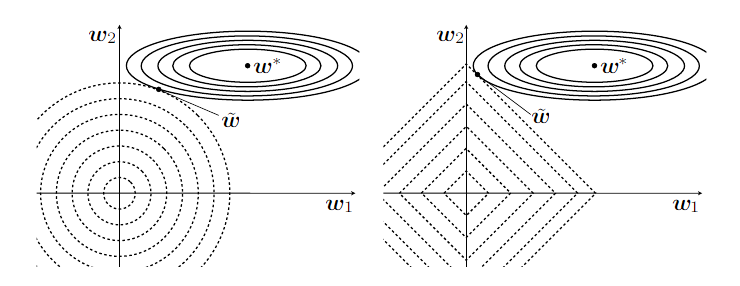
\includegraphics[width=0.8\linewidth]{images/4_regularizer}
\caption[]{Effekt der $L^2$- (links) und $L^1$-Norm (rechts) auf den Wert der optimalen Gewichte $W$ mit empirischem Optimum $W^*$ \cite[vgl.][Kap. 7.2, S. 199]{Bengio2015}}.
\label{fig:4_regularizer}
\end{figure}


\subsubsection{$L^1$-Norm}

Bei der Verwendung der $L^1$-Norm zur Berechnung von $\Omega(\Theta)$ bleibt nach dem Ableiten lediglich das Vorzeichen $sign(w_i)$ der einzelnen Gewichte übrig. Damit ergibt sich die in Gleichung \ref{eq:reg1} dargestellte Regel für die Berechnung des neuen Gradienten $\nabla_w \hat{J}(W,b)$ pro Gewicht $w$ \cite[vgl.][Kap. 7.2, S. 203 f.]{Bengio2015}. 

\begin{equation}
\label{eq:reg1}
\nabla_w \hat{J}(W,b) = \nabla_w J(W,b) + \alpha sign(w)
\end{equation}

Die $L^1$-Regu\-lari\-sierung bestraft die Summe aller Absolutwerte der Gewichte und verkleinert diese somit  während des Gradientenabstiegs stetig mit gleicher Rate. Die rechte Grafik in Abbildung \ref{fig:4_regularizer} zeigt, dass $L^1$-Regu\-lari\-sierung einerseits zu größeren Werten führt, im Gegenzug jedoch auch sehr kleine Werte bevorzugt. Diese Eigenschaft führt zu \textit{Sparsity}, da kleine Gewichte $w$ zwangsläufig im Laufe des Trainings den Wert Null annehmen \cite[vgl.][Kap. 7.2, S. 203]{Bengio2015}.
Die bayesianische Interpretation der Methode ist die A-priori Annahme einer isotropischen Laplace-Verteilung der Gewichte \cite[vgl.][Kap. 7.2, S. 206]{Bengio2015}.

\subsubsection{$L^2$-Norm}
\label{ch:l1_l2}
Trotz der interessanten \textit{Sparsity} Eigenschaften der $L^1$-Regularisierung wird im Deep Learning meist die $L^2$-Norm zur Regularisierung  verwendet und die \textit{Sparsity} mit ReLu-Funktionen erzwungen \cite[vgl. z.B.][]{Krizhevsky2012}.
Diese aus der \textit{Ridge Regression} bekannte Form der Regularisierung, führt zu Parameterwerten näher dem Ursprung. In der bayesianische Interpretation entspricht diese somit einer Gauß-Verteilung mit Mittelwert Null \cite[vgl.][Kap. 7.2, S. 200]{Bengio2015}. Der Gradient der $L^2$ regularisierten Fehlerfunktion ist in Gleichung \ref{eq:reg2} aufgeführt.

\begin{equation}
\label{eq:reg2}
\nabla_w \hat{J}(W,b) = \nabla_w J(W,b) + \alpha w
\end{equation}

Diese Form der Regularisierung führt dazu, dass das Modell eine größere Varianz in den Trainingsdaten $X$ annimmt. Somit werden Gewichte zu Merkmalen mit geringer Kovarianz zur Ausgabe verkleinert \cite[vgl.][Kap. 7.2, S. 200 f.]{Bengio2015}. Die \textit{Ridge Regression} in Gleichung \ref{eq:reg3} verdeutlicht diesen Aspekt, indem ein Vielfaches der Identitätsmatrix $I$ auf die Kovarianzmatrix $X^TX$ addiert wird.

\begin{equation}
\label{eq:reg3}
w = (X^TX + \alpha I)^{-1} X^Ty
\end{equation}


In Abbildung \ref{fig:4_regularizer} erkennt man diesen Effekt daran, dass das Gewicht $w_1$, in dessen Richtung die Zielfunktion im Gewichtsraum eher flach ist, geschrumpft wird.

\subsubsection{Max-$L^2$-Norm}

Max-$L^2$-Norm Regularisierung beschreibt eine Methode, welche die $L^2$-Norm der Gewichte eines Neurons $p$ beschränkt sodass $||w_p||_2 <= c$ gilt. Werte für den Hyperparameter $c$ liegen meist zwischen $3$ und $4$ \cite[vgl.][]{Srivastava2014}. Diese Art der Regularisierung projiziert folglich die Gewichte eines Neurons $w_p$ auf eine Kugel mit Radius $c$, sobald die Norm diese verlässt. 
Nach \cite{Srivastava2014} verhindert dies den \textit{Exploding Gradient}-Effekt, da die Gewichte den Fehler beim Rückpropagieren nicht mehr überproportional verstärken können. Dies ermöglicht größere Lernraten im Vergleich zum Training ohne Max-Norm-Re\-gu\-la\-ri\-sie\-rung, was gerade in Verbindung mit Dropout-Learning (siehe Kapitel \ref{ch:dropout}) von Vorteil ist, da so größere Gebiete im Gewichtsraum untersucht werden können.

\begin{figure}[H]
\centering
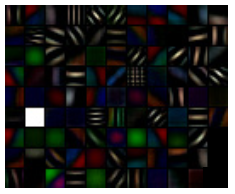
\includegraphics[width=0.4\linewidth]{images/4_max_norm}
\caption[]{Ein dominierender Filter ohne Max-Norm Regularisierung  \cite[siehe][]{Zeiler2014}}.
\label{fig:4_max_norm}
\end{figure}

 Abbildung \ref{fig:4_max_norm} zeigt einen weiteren Grund für die Notwendigkeit dieser Form der Regularisierung. Die Dominanz eines Filters über alle anderen kann effektiv verhindert werden \cite[vgl.][]{Zeiler2014}.




\subsection{Modellkapazität}
Beim Training großer Modelle mit hoher Kapazität ist \textit{Overfitting} von zentraler Bedeutung. \textit{Overfitting} beschreibt den Effekt eines kleiner werdenden Fehlers auf den Trainingsdaten bei gleichzeitiger Verschlechterung der Performanz auf den Testdaten. Abbildung \ref{fig:4_overfitting} stellt diesen Effekt grafisch dar.

\begin{figure}[H]
\centering
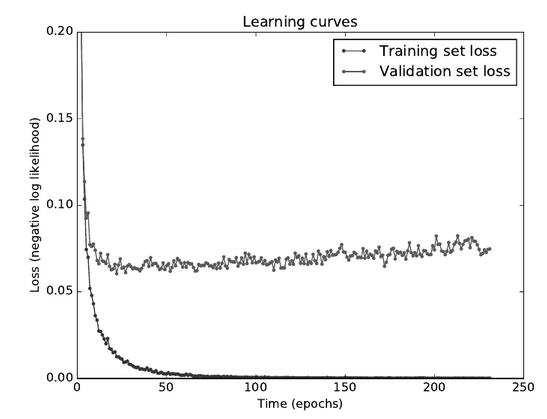
\includegraphics[width=0.4\linewidth]{images/4_overfitting}
\caption[]{\textit{Overfitting} am Beispiel des MNIST-Datensatzes \cite[siehe][Kap. 7.3, S. 216]{Bengio2015} }.
\label{fig:4_overfitting}
\end{figure}

Im Folgenden werden Methoden zusammengefasst, welche die Kapazität des Modells regulieren und damit aktiv versuchen \textit{Overfitting} zu verhindern.



\subsubsection{Early Stopping}
Die einfachste, sehr häufig angewandte Methode \textit{Overfitting} aktiv zu verhindern, ist das sogenannte \textit{Early Stopping}. Diese Methode teilt die Trainingsmenge zuerst in zwei Teilmengen. Sie setzt somit einen Satz Validierungsdaten voraus \cite[vgl. hierzu und im Folgenden][Kap. 7.3, S. 216 ff.]{Bengio2015}.

Beim \textit{Early Stopping} wird während des Trainings in regelmäßigen Abständen der Fehler auf den Validierungsdaten beobachtet. Verbessert sich dieser, werden die aktuellen Gewichte und Schwellwerte des Modells gesondert gespeichert. Am Ende des Trainings werden folglich nicht die aktuellsten Gewichte zurück\-gegeben sondern diejenigen, welche den kleinsten Validierungsfehler erzeugten.
Anstelle eines lokalen Minimums über den Trainingsdaten wird somit ein lokales Minimum des Validierungsfehlers gesucht. Das Training stoppt, sobald sich der Validierungsfehler über mehrere Epochen nicht verbessert hat (\textit{Early Stopping Patience}). Die Kapazität des Modells wird dahingehend beschränkt, dass die Trainingszeit limitiert ist.
Bei der $L^2$-Regularisierung wurde beobachtet, dass Gewichte in Richtungen hoher Krümmung hinsichtlich der Zielfunktion weniger stark reguliert werden als andere. Diese Beobachtung lässt laut \cite{Bengio2015} eine Ähnlichkeit zum \textit{Early Stopping} erkennen, da die Gewichte in Verbindung mit hoher Krümmung relativ zu den anderen Gewichten früher im Trainingsprozess gelernt werden.

\subsubsection{Parameteranzahl limitieren}
Die Kapazität des Modells lässt sich ebenso durch Vereinfachung beziehungsweise Verkleinerung und somit einer Verringerung der zu lernenden Gewichte regulieren. Im Umfeld des Deep Learning werden grundsätzlich zwei verschiedene Methoden beschrieben: Teilen der Gewichte (\textit{Parameter Sharing}) und Reduktion der Verbindungen zwischen Merkmalen. \\

\textit{Parameter Sharing} \\
Diese Methode ist am meisten verbreitet in CNNs und die Grundlage für die großen Erfolge im maschinellen Lernen und Deep Learning. CNNs berechnen an verschiedenen Stellen des Eingabebeispiels mit den selben Gewichten eine gewichtete Summe, was der algebraischen Faltung entspricht \cite[vgl.][]{LeCun1998}. 
Durch \textit{Parameter Sharing} ist es möglich große neuronale Netze zu trainieren, ohne die Trainingsmenge entsprechend zu vergrößern. Damit sind CNNs ein herausragendes Beispiel für die Integration von Expertenwissen in einem neuronalen Netz \cite[vgl.][Kap 7.8, S. 224]{Bengio2015}. \\

\begin{figure}
\centering
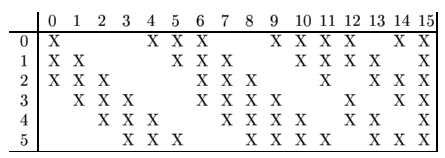
\includegraphics[width=0.4\linewidth]{images/4_connections}
\caption[]{Verbindungsmatrix der Merkmale beziehungsweise \textit{Feature-Maps} (Zeilen) mit den dazugehörigen Gewichten beziehungsweise Faltungsmasken (Spalten) zweier aufeinanderfolgenden Schichten \cite[siehe][]{LeCun1998}}.
\label{fig:4_connections}
\end{figure}

\begin{figure}
\centering
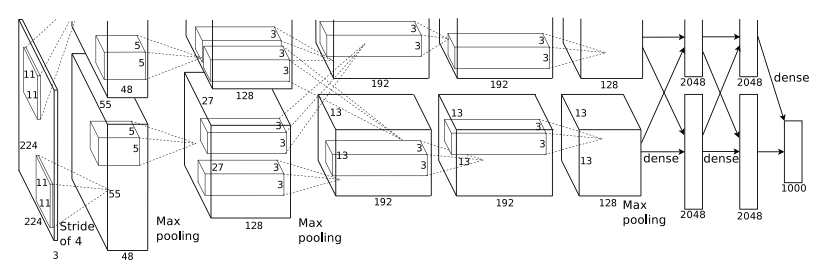
\includegraphics[width=0.9\linewidth]{images/4_Kriz}
\caption[]{Architektur für \textit{ImageNet 2012} mit limitierten Verbindungen zwischen \textit{Feature-Maps} zwecks Parallelisierung  \cite[siehe][]{Krizhevsky2012}}.
\label{fig:4_Kriz}
\end{figure}

\textit{Limitierung von Verbindungen zwischen Merkmalen} \\
Bei Nutzung diese Methode wird ebenfalls das Ziel verfolgt Parameter zu reduzieren, wobei allerdings ein anderer Ansatz als bereits vorgestellt gewählt wird. Anstatt die Eingabe nur in über\-lapp\-ende, rezeptive Felder zu unterteilen und mit den selben Gewichten zu gewichten, werden zusätzlich die unterschiedlichen Dimensionen der Eingabe (z. B. RGB-Kanäle) überlappend aufgeteilt. Die bekannte Verbindungsmatrix von \textit{LeNet 5} ist zur Veranschaulichung in Abbildung \ref{fig:4_connections} dargestellt.
Neben der Reduktion von zu trainierenden Gewichten erlaubt dies auch eine bessere Extraktion unabhängiger Merkmale \cite[vgl.][]{LeCun1998}. Darüber hinaus bedient sich die Architektur von \cite{Krizhevsky2012} zwecks Parallelisierung des Netzes auf mehrere Rechenkerne (hier GPUs) derselben Methode, wie Abbildung \ref{fig:4_Kriz} zeigt.\\


\subsubsection{Dropout}
\label{ch:dropout}
Die Dropout-Methode wurde von \cite{Hinton2012} eingeführt und bezeichnet eine Methode, mehrere kleinere Modelle zu lernen und die verschiedenen Ausgaben zu kombinieren (\textit{Model Averaging}). Hierbei ist hervorzuheben, dass dies gleichzeitig und in einem neuronalen Netz geschieht. \cite[vgl.][]{Srivastava2014}.

Die Dropout-Methode wurde mit dem Ziel entwickelt MLPs wenigen Trainingsdaten zu trainieren, was typischerweise in \textit{Overfitting} resultiert. Hierbei soll die Architektur des Netzes im Training zufällig für jedes Trainingsbeispiel verändert werden, um Abhängigkeiten (\textit{Co-Adaptions}) extrahierter Merkmale zu vermeiden \cite[vgl.][]{Hinton2012}. Dazu werden zufällig einzelne Neuronen deaktiviert. Dieses Grundprinzip ist in Abbildung \ref{fig:4_dropout} dargestellt. Um den Gradienten richtig zu berechnen, ist es wichtig, dass die deaktivierten Neuronen auch im Backpropagation beim \textit{Backward Pass} deaktiviert bleiben.

Wird das zufällige ausschalten von Neuronen deaktiviert, existiert ein trainiertes Netz, welches implizit mehrere Modelle kombiniert und somit eine deutliche Verbesserung gegenüber bestehenden Regularisierungsmethoden hinsichtlich \textit{Overfitting} darstellt \cite[vgl.][]{Srivastava2014}. Damit die Gewichte durch die Kombination der Modelle im Testlauf nicht zu groß sind, müssen diese mit ${1-p}$ skaliert werden. 
Als Hyperparameter muss für Dropout lediglich die Wahrscheinlichkeit $p$ ein Neuron zu deaktivieren angegeben werden. Typische Werte reichen von $0.1$ bis $0.5$ (vgl. \cite{Krizhevsky2012}, \cite{Srivastava2014} oder \cite{Simonyan2014}).

Wird die Standardinitialisierung in Verbindung mit ReLu-Funk\-tionen verwendet, muss darauf geachtet werden, dass die Neuronen positive Ausgaben erzeugen, um ebenso positive Gradienten für das Lernen zu erhalten. Dies kann mittels des Schwellwertes $b=1$ oder einer hinreichend großen Varianz erreicht werden \cite[vgl.][]{Hinton2012}.

Die beschriebene Methode kann auch bestehende, gut funktionierende Netze verbessern. Da die effektive Kapazität durch Dropout verringert wird, ist es sinnvoll die Anzahl existierender Neuronen $n$ auf $n/(1-p)$ zu erhöhen \cite[vgl.][]{Srivastava2014}. Aufgrund der Tatsache, dass CNNs die Modellkapazität durch \textit{Parameter Sharing} bereits stark regulieren, ist Dropout in Convolution-Layer nicht gleichermaßen effektiv wie in Hidden-Layer \cite[vgl.][]{Hinton2012}.	

\begin{figure}
\centering
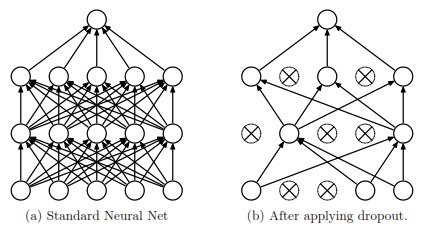
\includegraphics[width=0.6\linewidth]{images/4_dropout}
\caption[]{Schematische Darstellung eines gewöhnlichen MLP (links) und eines Dropout-MLP (rechts) \cite[siehe][]{Srivastava2014}}.
\label{fig:4_dropout}
\end{figure}			
	
\subsubsection{Padding im Convolution-Layer}
Wird in den Convolution-Layern die Eingabe bzw. die Ausgabe an den Rändern mit $(K - 1) / 2$ Nullen erweitert (Padding), verändert der Convolution-Layer nicht die Größe der Eingaben. Gerade bei der Verwendung von großen Filtermasken, wie beispielsweise $K = 7$, verhindert diese Methode eine schnelle Verkleinerung der Größe der Ausgabe. Damit wird auch verhindert, dass die Informationen an den Rändern der Eingabe früh im Netz verblassen \cite[vgl.][]{Kaparthy2014}. \\
		
				
\subsection{Erweitern der Trainingsdaten}
Die Kapazität eines Modells ist im Allgemeinen eine relative Größe basierenden auf der zur Verfügung stehenden Trainingsmenge. Folglich lässt sich das Problem des \textit{Overfittings} auch umgekehrt formulieren: Anstatt die Kapazität zu regulieren, kann die Menge der Trainingsdaten erhöht werden. Diese Methode wird häufig als \textit{Data Augmentation} bezeichnet und umfasst drei Bereiche: Affine Transformationen, Elastische Transformationen und Additives Rauschen. Diese Formen der Regularisierung haben oftmals großen Einfluss auf die Performanz des Systems hinsichtlich Invarianzen und müssen deshalb beim Vergleich unterschiedlicher Algorithmen und Lernmaschinen berücksichtigt werden.
\cite[vgl.][Kap. 7.5, S. 210 f.]{Bengio2015}



\subsubsection{Affine Transformationen}
Affine Transformationen können die Generalisierung des Netzes immens verbessern. Eingaben sollen hierbei so verändert werden, dass gewünschte Invarianzen besser trainiert werden. Dies ist auch dann von Vorteil, wenn das Modell selbst bereits gewisse Invarianzen, wie beispielsweise die Translationsinvarianz von CNNs, enthält. So finden affine Transformationen Anwendung im Training von \textit{LeNet 5} von \cite{LeCun1998} und im \textit{AlexNet} von \cite{Krizhevsky2012}.
Eine analytische Methode \textit{Data Augmentation} in den Trainingsprozess einzubauen, beschreibt \cite{Simard92} mittels des Tangent-Prop-Algorithmus.


\subsubsection{Elastische Transformationen}
Elastische Transformationen erweitern das Set an verfügbaren affinen Operationen und verbessern die Generalisierung dadurch weiter. 
Zunächst wird ein Vektorfeld pro Dimension generiert, welches zufällige Verschiebungen der einzelnen Eingabemerkmale (z. B. Pixel) beschreibt. Die generierten Felder werden anschließend mit einem Gauß-Kern gefaltet, beziehungsweise weichgezeichnet, und auf die originale Eingabe angewandt \cite[vgl.][]{Simard2003}.
Das Ergebnis elastischer Transformationen ist in Abbildung \ref{fig:4_elastic} dargestellt.

\begin{figure}
\centering
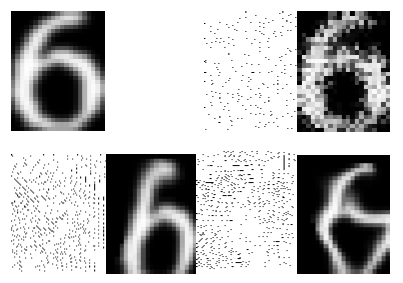
\includegraphics[width=0.5\linewidth]{images/4_elastic}
\caption[]{Originale Eingabe (oben links) und drei Beispiele elastisch veränderter Eingaben mit zugehörigem Vektorfeld \cite[siehe][]{Simard2003}}.
\label{fig:4_elastic}
\end{figure}


\subsubsection{Additives Rauschen}
Eine weitere Möglichkeit das System robuster zu machen, ist das Training mit additivem Rauschen. So korrumpiert beispielsweise \cite{Vincent2008} die Trainingsdaten zu einem gewissen Grad mit additiven Rauschen, Maskierung oder \textit{Salt-and-Pepper} und konstruiert damit einen \textit{Denoising Autoencoder} (DAE). Mehrere DAEs bilden zusammen \textit{Stacked Denoising Autoencoder} und schließen damit die Lücke zu den beschränkten Boltzmann-Maschinen und (DBNs) im Bereich des unüberwachten Vortrainings \cite[vgl.][]{Vincent2010}.

Gerade die Maskierung einzelner Merkmale im Eingaberaum liefert die Grundlage für das spätere Dropout, welches sowohl für die Hidden-Layer als auch im Input-Layer geeignet ist und die Generalisierung deutlich verbessern kann \cite[vgl.][]{Srivastava2014}.


\section{Visualisierungsmethoden}
Gerade die Verbindung von Bilderkennung und CNNs macht die Anwendung von Visualisierungsmethoden besonders attraktiv, da sich gewisse Verhaltensweisen des neuronalen Netzes so besser verstehen lassen.
Die meisten der vorgestellten Methoden haben das Ziel der Kritik, \textit{Features} aus neuronalen Netzen ließen sich nicht interpretieren, entgegenzuwirken \cite[vgl.][]{Zeiler2014}.

\subsection{Primitiv}

Die einfachste Möglichkeit des Sichtbarmachens des Neuronalen Netzes, ist die Visualisierung der Ausgabe beziehungsweise der Gewichte und wird deshalb als primitiv bezeichnet. Dennoch können diese Techniken wichtige Einblicke gewähren.

\subsubsection{Neuronen-Aktivierung}

Die Visualisierung der Ausgabe eines \textit{AlexNet} von \cite{Krizhevsky2012} ist in Abbildung \ref{fig:4_output} (links) dargestellt. Die Eingabe ist ein Bild einer Katze. Es fällt sofort auf, dass die Aktivierungen sehr dünnbesetzt (\textit{sparse}) sind, was letztendlich auf die ReLu-Funktionen zurückzuführen ist \cite[vgl.][]{Glorot2011}.

\begin{figure}
\centering
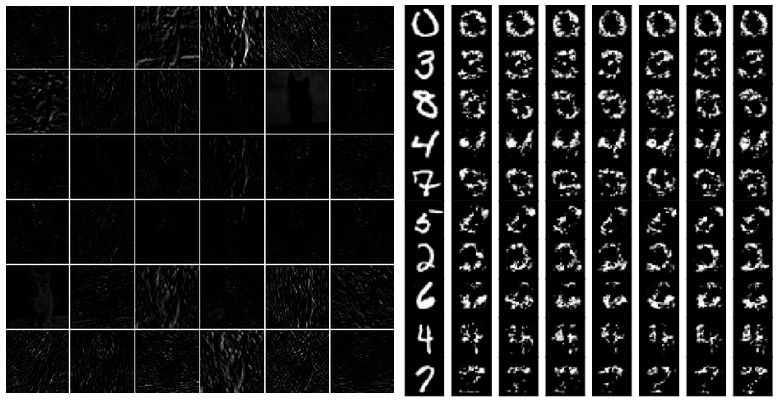
\includegraphics[width=0.6\linewidth]{images/4_output}
\caption[]{Aktivierungen des \textit{AlexNet} nach erstem Layer (links)  \cite[siehe][]{Kaparthy2014} und Rekonstruktionen eines Autoencoders (rechts) \cite[siehe][]{Vincent2010}}.
\label{fig:4_output}
\end{figure}

Diese Visualisierungsmethode kann in mehrerer Hinsicht unterstützen. Einerseits können so tote Neuronen identifiziert werden (vgl. \textit{Dying ReLu}-Effekt in \cite{Maas2013}). Andererseits kann überprüft werden, ob die Aktivierungen die gewünschte \textit{Sparsity} und Lokalität aufweisen.
Wird ein Autoencoder verwendet, kann darüber hinaus interessant sein, die Aktivierung beziehungsweise Ausgabe des Netzes zu visualisieren, da diese der Rekonstruktion der Eingabe entsprechen. Abbildung \ref{fig:4_output} (rechts) zeigt derartige Rekonstruktionen auf dem MNIST-Datensatz.

\subsubsection{Faltungskerne}
%http://eric-yuan.me/cnn/

Eine weitere einfache Möglichkeit, Informationen über das CNN zu erhalten ist die Visualisierung der gelernten Filtermasken. Abbildung \ref{fig:4_kernel} zeigt die Faltungskerne des ersten Layers eines trainierten \textit{AlexNet}. 

\begin{figure}[H]
\centering
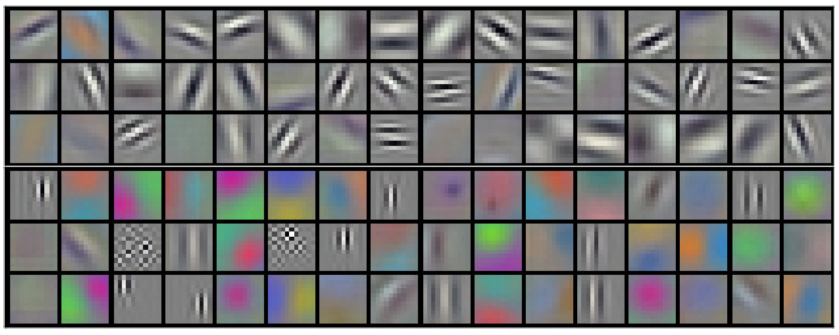
\includegraphics[width=0.5\linewidth]{images/4_kernel}
\caption[]{Die Faltungskerne des ersten Layers eines trainierten \textit{AlexNet}  \cite[siehe][]{Krizhevsky2012}}.
\label{fig:4_kernel}
\end{figure}

Trainierte Netze haben typischerweise glatte, Gabor-Filtern ähnliche Filtermasken. Verrauschte Filtermasken können hingegen entweder ein Indikator für eine fehlende Regularisierung und damit einhergehendes \textit{Overfitting} sein oder darauf hinweisen, dass das Netz nicht ausreichend konvergiert ist \cite[vgl.][]{Kaparthy2014}.     


\subsection{Gradientenbasiert}

Eine weitere Klasse von Visualisierungsmethoden arbeiten auf Basis des Backpropagation-Algorithmus. Dies bedeutet, dass sie sich der Fehler\-rück\-führung (\textit{Backward Pass}) bedienen und diese zur Visualisierung verwenden.

\subsubsection{Neuronen-Visualisierung}
Die erste Methode ist die sogenannte Deconvnet-Visualisierung von \cite{Zeiler2014}. Diese kann als Neuronen-Visualisierung bezeichnet werden, da letztlich Aktivierungen einzelner Neuronen visualisiert werden. Die Grundidee des Verfahrens ist es, einzelne Aktivierungen im Netz im Eingaberaum sichtbar zu machen. Dazu wird ein bestimmtes Neuron beziehungsweise eine bestimmte \textit{Feature-Map} ausgewählt und die Aktivierungen werden über die gesamte Testmenge gemessen. Die Beispiele mit den höchsten Aktivierungen werden gespeichert. Im Anschluss nutzt die Visualisierung diese Beispiele und rekonstruiert die erzeugten Aktivierungen, indem alle anderen \textit{Feature-Maps} dieses Layers Null gesetzt werden. Für die Rekonstruktion $R$ der Aktivierung wird im Grunde die Fehlerrückführung des Backpropagation-Algorithmus verwendet. Damit gilt in einem Convolution-Layer die Gleichung \ref{eq:zeiler1} zur Rekonstruktion einer Feature-Map.

\begin{equation}
\label{eq:zeiler1}
R^l_j = \sum_{i = 0}^{n} \hat{R}^{l+1}_{i} \ast rot180(W_{ij})
\end{equation}

Im Unterschied zur Berechnung des Gradienten mit Backpropagation, wird bei diesem Verfahren die Aktivierungsfunktion nicht abgeleitet. Stattdessen wird die Aktivierungsfunktion $\phi$ selbst mit der Rekonstruktion $R^{l+1}$ im Sinne des \textit{Forward Pass} berechnet. Formel \ref{eq:zeiler2} verdeutlicht diesen Zusammenhang für den Layer $l$.

\begin{equation}
\label{eq:zeiler2}
\hat{R}^{l+1}_i = \phi_l(R^{l+1}_i)
\end{equation}

Eine weitere Besonderheit stellen die Pooling-Layer dar, da diese im Prinzip nicht umkehrbar sind. Die von \cite{Zeiler2014} vorgeschlagene Methode sieht deshalb lediglich die Variante Max-Pooling vor und verbietet alle anderen Pooling-Verfahren. Max-Pooling bietet hierbei den Vorteil, dass im \textit{Forward Pass} die Stellen der Maxima vermerkt werden.

\begin{figure}
\centering
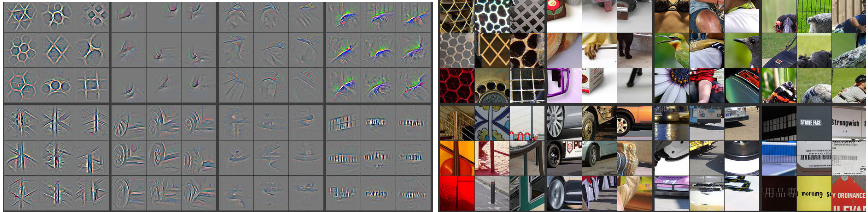
\includegraphics[width=0.9\linewidth]{images/4_zeiler}
\caption[]{Mit Deconvnet rekonstruierte Aktivierungen im dritten Layer (links) und dazugehörige originale Eingabebilder (rechts) \cite[siehe][]{Zeiler2014}}.
\label{fig:4_zeiler}
\end{figure}

Acht ausgewählte Neuronen im dritten Layer mit den jeweiligen zur höchsten Aktivierung korrespondierenden Eingabebildern, sind in Abbildung \ref{fig:4_zeiler} dargestellt.

\subsubsection{Saliency-Visualisierung}
%Gerneralized
Die sogenannte Saliency-Visualisierung von \cite{Simonyan2013} ist dem Deconvnet-Verfahren im Grunde sehr ähnlich. Es unterscheidet sich allerdings in einem zentralen Punkt. 
Während das Verfahren von \cite{Zeiler2014} Veränderungen im Vergleich zum Backpropagation-Algorithmus vornimmt, hält sich dieses Verfahren strikt an die Fehlerrückführung und berechnet damit die Ableitungen der Aktivierungsfunktionen, wie Formel \ref{eq:simonyian} zeigt. 

\begin{equation}
\label{eq:simonyian}
\hat{R}^{l+1}_i = R^{l+1}_i \circ \phi^{'}(z_i)
\end{equation}

Dies bietet den Vorteil, dass sich das Verfahren somit sowohl auf die Convo\-lution-Layer als auch die Hidden-Layer anwenden lässt. Dies lässt sich damit begründen, dass das Verfahren im ursprünglichen Sinne einzelne Klassen im Eingaberaum visualisiert \cite[vgl.][]{Simonyan2013}.


\begin{figure}
\centering
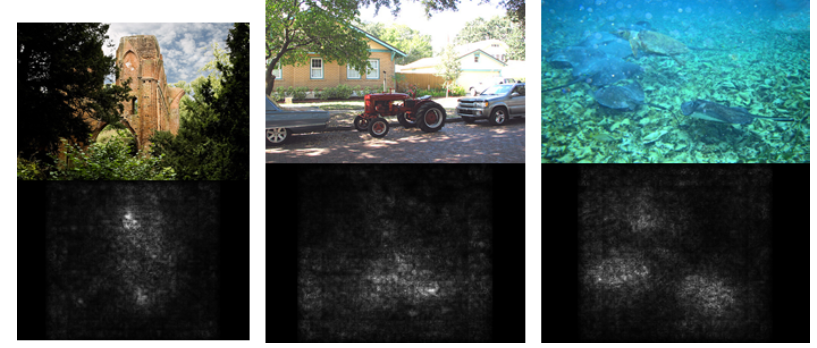
\includegraphics[width=0.6\linewidth]{images/4_simonyan}
\caption[]{Originale Eingabebilder (oben) und dazu gehörige \textit{Saliency-Maps} (unten) \cite[siehe][]{Simonyan2013}}.
\label{fig:4_simonyan}
\end{figure}

Abbildung \ref{fig:4_simonyan} zeigt die beschriebene Technik, angewandt auf Beispiele aus dem \textit{ImageNet}-Datensatz. Die \textit{Saliency-Map} zeigt die Rekonstruktion der entsprechenden Aktivierung im Output-Layer. 

\subsection{Nachverarbeitung}
Methoden im Bereich Nachverarbeitung sind dadurch charakterisiert, dass ein trainiertes MLP, beziehungsweise CNN, lediglich zur Erzeugung von Merkmalsvektoren oder zur Berechnung von Ausgaben herangezogen wird. Diese Art der Visualisierung beschränkt sich demnach auf den Kontext und betrachtet das Netz als \textit{Blackbox}, beziehungsweise als eine Funktion $h(x)$.


\subsubsection{t-SNE}

Die Methode t-Distributed Neighbor Embedding (t-SNE) beschreibt ein von \cite{Laurens2008} entwickeltes Optimierungsverfahren zur Dimensionsreduktion. Es verbessert das klassische SNE-Verfahren insofern, dass die Gradienten für die Optimierung einfacher zu berechnen sind. Darüber hinaus wird anstelle einer Gauß- eine Student-t-Verteilung als Ähnlichkeitsmaß im niedrigdimensionalen 2D oder 3D Zielraum verwendet \cite[vgl.][]{Laurens2008}. Der Grundmechanismus von t-SNE ist die Minimierung des Unterschieds zweier Wahrscheinlichkeitsverteilungen (Kullback-Leibler-Divergenz): Der Wahrscheinlichkeitsverteilung von Paaren im hochdimensionalen $P$ Raum sowie der im niedrigdimensionalen Raum $Q$. Damit ergibt sich die zu minimierende Zielfunktion $C$ in Formel \ref{eq:tsne}.


\begin{equation}
\label{eq:tsne}
C = KL(P||Q) ) = \sum_{i}^{} \sum_{j}^{} p_{ij} log(\frac{p_{ij}}{q_{ij}})
\end{equation}


\begin{figure}
\centering
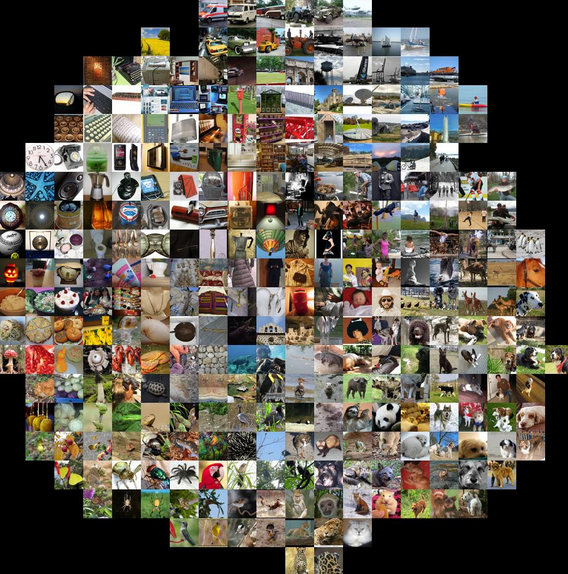
\includegraphics[width=0.5\linewidth]{images/4_t_sne}
\caption[]{t-SNE Einbettung einer Auswahl an \textit{ImageNet}-Bildern auf Basis der Aktivierung des letzten Layers im \textit{AlexNet} (Bild: Laurens van der Maaten, Facebook AI Research)}.
\label{fig:4_t_sne}
\end{figure}


Grundsätzlich können die von neuronalen Netzen erzeugten Merkmalsvektoren (\textit{Features}) auch mittels der Hauptkomponentenanalyse (PCA) visualisiert werden. Die t-SNE unterscheidet sich von PCA allerdings in einigen zentralen Eigenschaften \cite[vgl. hierzu und im Folgenden][]{Laurens2008}:

\begin{itemize}
\item Wenn ein Großteil der Varianz nicht in den ersten zwei, beziehungsweise drei, Hauptkomponenten beschrieben ist, kann t-SNE bessere Ergebnisse liefern, da es versucht die gesamte Information abzubilden.
\item t-SNE ist im Vergleich zur PCA keine orthogonale, lineare Transformation sondern eine nichtlineare Reduktion mit nicht zwingend orthogonalen Komponenten.
\item t-SNE findet, aufgrund der nicht-konvexen Zielfunktion, nicht immer zum globalen Minimum.
\item t-SNE ist darauf spezialisiert hochdimensionale Daten auf maximal zwei beziehungsweise drei Dimensionen zu reduzieren.
\end{itemize}



Abbildung \ref{fig:4_t_sne} zeigt die t-SNE 2D-Transformation des Merkmalsvektors vor dem Output-Layer eines \textit{AlexNet}. Als Eingabedaten dient eine Teilmenge des \textit{ImageNet}-Datensatzes. Diese Art der Visualisierung zeigt, dass das CNN Merkmale extrahiert und darauf aufbauend relevante von irrelevanten Merkmalen trennen kann. Dies lässt sich sehr deutlich daran erkennen, dass inhaltlich ähnliche Bilder näher zusammen sind als andere und somit Kategorien oder Gruppen und nicht Hintergrund oder Färbung die Daten charakterisieren \cite[vgl.][]{Bell2015}.


\begin{figure}
\centering
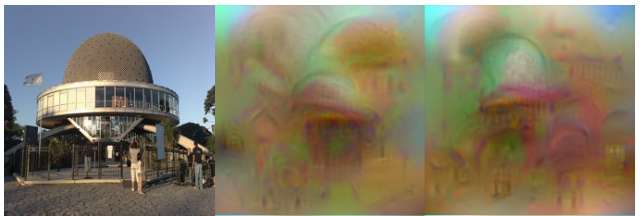
\includegraphics[width=0.5\linewidth]{images/4_inceptionismb}
\caption[]{Mögliche Rekonstruktionen des originalen Eingabebilds (oben links) \cite[siehe][]{Simard2003}}.
\label{fig:4_inceptionism}
\end{figure}

\subsubsection{Inceptionism}
Ein weiteres Verfahren, welches als \textit{Inceptionism}\footnote{Das Kunstwort \textit{Inceptionism} geht auf einen Blog-Eintrag von \textit{Research at Google} zurück (\url{http://googleresearch.blogspot.de/2015/06/inceptionism-going-deeper-into-neural.html} (26.08.2015)).} bezeichnet wird, wählt eine andere Herangehensweise. Durch Nutzung dieses Verfahrens wird versucht, ausgehend von einer Aktivierung, beziehungsweise einem Merkmalsvektor eines Layers, eine dazu passende Eingabe zu rekonstruieren. 
Das Grundverfahren, um Merkmalsvektoren zu invertieren, stammt von \cite{Mahendran2014}. Dieses Verfahren nimmt ein beliebiges Eingabebild $x_0$ und berechnet mittels eines trainierten CNN die Ausgabe $h_0 = h_l(x_0)$ in einem beliebigen Layer $l$. Das Ziel des Verfahrens ist es, die Zielfunktion $C$ in Gleichung \ref{eq:incept} mit Regularisierer $R(x)$ zu minimieren und ausgehend vom Rauschen ein optimales $x$ zu finden. 

\begin{equation}
\label{eq:incept}
C = ||h(x) - h_0||^2 + \lambda R(x)
\end{equation}

Der Regularisierer sorgt dafür, dass das optimale $x$ innerhalb eines für Bilder üblichen Intervalls $B = [-128,128]$ liegt (Formel \ref{eq:incept1}) und das resultierende Bild stückweise konstant ist (Formel \ref{eq:incept2}).

\begin{equation}
\label{eq:incept1}
R_1 = ||x||^6_6
\end{equation}

\begin{equation}
\label{eq:incept2}
R_2 = \sum_{i,j}^{} [(x_{i,j+1} - x_{ij})^2 + (x_{i+1,j} - x_{ij})^2)]^{\frac{1}{2}}
\end{equation}


Abbildung \ref{fig:4_inceptionism} zeigt fünf Optimierungen auf Basis des Eingabebilds oben links.


